\documentclass[letterpaper,11pt]{exam}
\usepackage[font=small, labelfont=bf]{caption}
\usepackage{amssymb,amsmath,amsthm,mathtools}
\usepackage{hyperref}
\usepackage{enumitem}
\usepackage{xcolor}
\usepackage{pdfpages}
\usepackage{amsmath}

\usepackage{graphicx}
\usepackage{subcaption}

\usepackage{booktabs}
\usepackage{caption}
\usepackage{multirow}

\usepackage{pythontex}
\usepackage{listings}
\usepackage{color}
\usepackage{floatflt}
\usepackage{listings}
\usepackage{xcolor}
\usepackage{ulem}

\setlength{\parskip}{1em}  % Space between paragraphs

\definecolor{dkgreen}{rgb}{0,0.6,0}
\definecolor{gray}{rgb}{0.5,0.5,0.5}
\definecolor{mauve}{rgb}{0.58,0,0.82}

\lstset{frame=tb,
  language=Java,
  aboveskip=3mm,
  belowskip=3mm,
  showstringspaces=false,
  columns=flexible,
  basicstyle={\footnotesize\ttfamily},
  numbers=none,
  numberstyle=\tiny\color{gray},
  keywordstyle=\color{blue},
  commentstyle=\color{dkgreen},
  stringstyle=\color{mauve},
  breaklines=true,
  breakatwhitespace=true,
  tabsize=4,
  frame=none
}

\lstset{
    language=C++,
    basicstyle=\ttfamily\footnotesize,
    keywordstyle=\color{blue},
    commentstyle=\color{gray},
    stringstyle=\color{red},
    % numbers=left,
    % numberstyle=\tiny\color{gray},
    stepnumber=1,
    numbersep=5pt,
    showspaces=false,
    showstringspaces=false,
    breaklines=true,
    frame=none,
    captionpos=b
}

\newcommand{\num}{3}
\newcommand{\topic}{Homework \num, Parallel VLSI Wire Routing via OpenMP}
\newcommand{\coursenum}{15-418/15-618}
\newcommand{\coursename}{\coursenum\ Parallel Computer Architecture and Programming}
\newcommand{\fullname}{Siqi Guo}
\newcommand{\andrew}{AndrewID: siqiguo}
\setlength{\parindent}{0pt} %don't indent first line of paragraph

\definecolor{lightblue}{rgb}{0.2, 0.7, 1} % Light blue in RGB
\hypersetup{
    colorlinks=true,        % Enable colored links (no boxes)
    linkcolor=lightblue,    % Color of internal links
    citecolor=lightblue,    % Color of citation links
    urlcolor=lightblue      % Color of external hyperlinks
}

\pagestyle{headandfoot}
\runningheader{\fullname}{\footnotesize \coursenum\ \textbf{\topic}}{\andrew}
\firstpagefooter{}{\thepage}{}
\runningfooter{}{\thepage}{}
\extrawidth{.5in}\extraheadheight{-.25in}

\begin{document}

\begin{center}
    {\LARGE\coursename\par}
    {\Large\topic\par}
    \fullname (\andrew) \hfill \today
\end{center}
\printanswers

\vspace{-0.2cm}
Use OpenMP to write parallel code using the shared address space model.
\vspace{-0.5cm}
\begin{itemize}[itemsep=0.1pt]
    \item Instrument the code to determine where the most time is spent in computation.
    \item Evaluate where optimizations are most valuable.
    \item Focus on avoiding sequential bottlenecks, memory contention, and workload imbalance.
\end{itemize}

First, let's visualize the VLSI wire routing.

\begin{figure}[h]
    \begin{minipage}{0.3\textwidth}
        \centering
        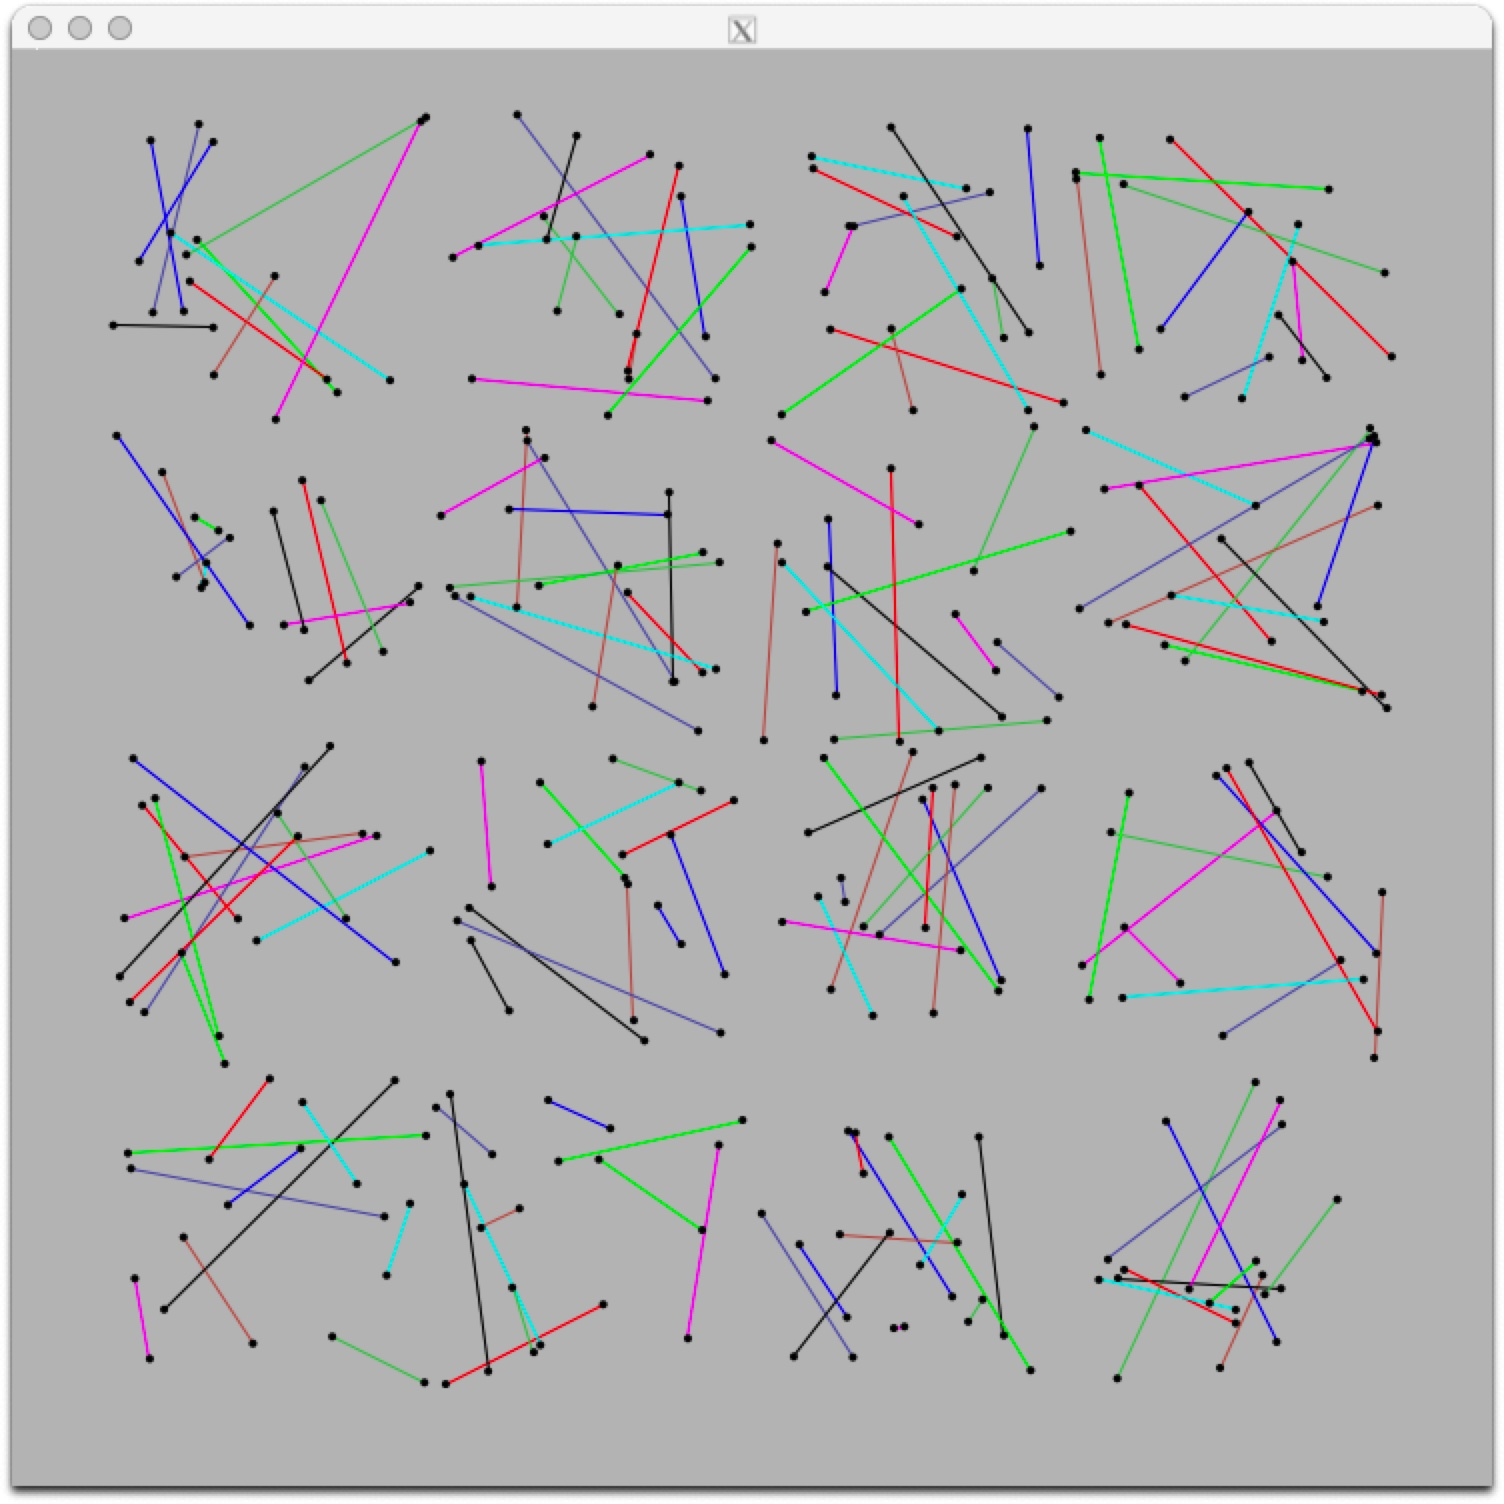
\includegraphics[width=\textwidth]{img/easy_4096.jpg}
        \label{fig:question1a}
        \subcaption{\texttt{java WireGrapher ./inputs/timeinput/easy\_4096.txt}}
    \end{minipage}
    \hspace{0.2cm}
    \begin{minipage}{0.3\textwidth}
        \centering
        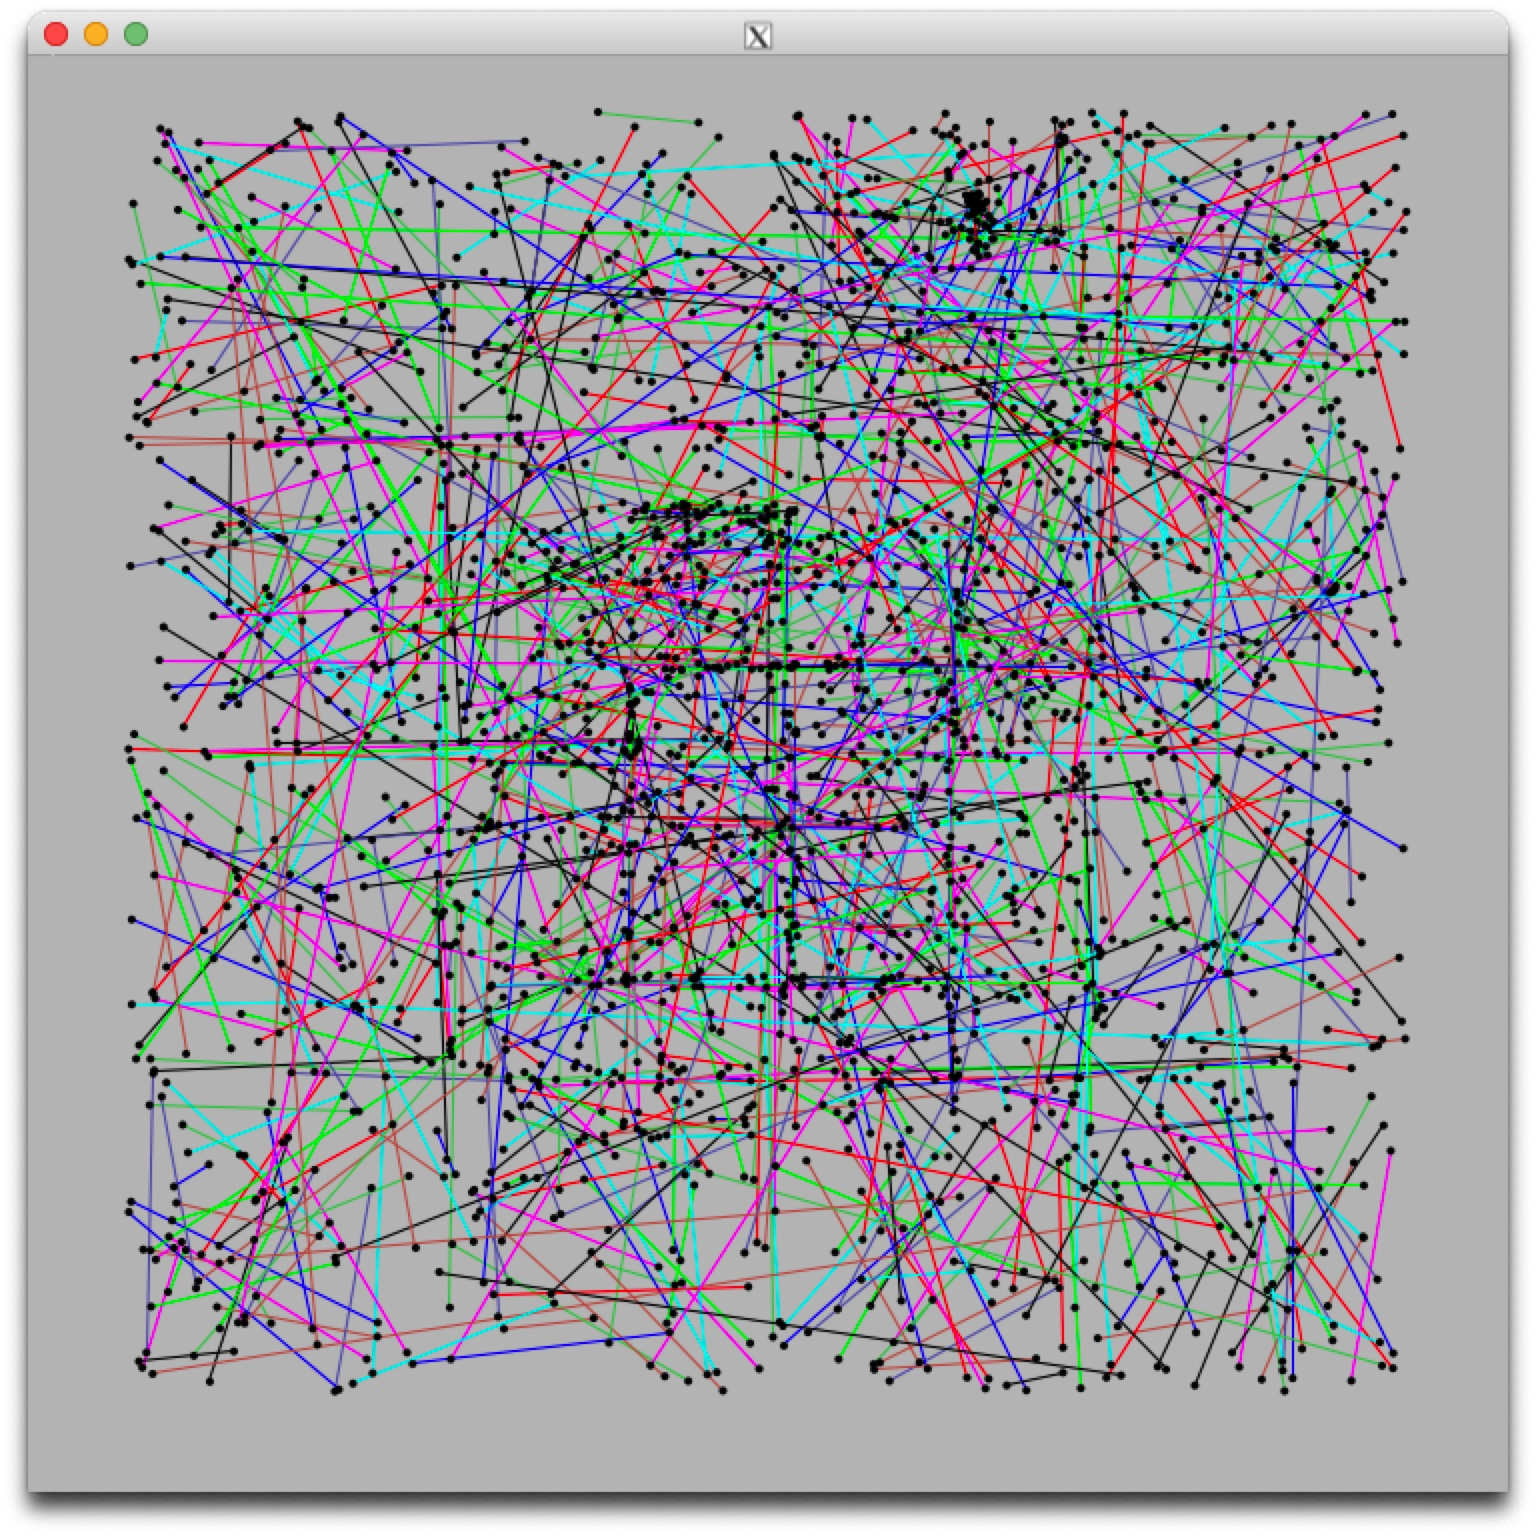
\includegraphics[width=\textwidth]{img/hard_4096.jpg}
        \label{fig:question1b}
        \subcaption{\texttt{java WireGrapher ./inputs/timeinput/hard\_4096.txt}}
    \end{minipage}
    \hspace{0.2cm}
    \begin{minipage}{0.3\textwidth}
        \centering
        
\includegraphics[width=\textwidth]{img/extreme_4096.jpg}
        \label{fig:question1b}
        \subcaption{\texttt{java WireGrapher ./inputs/timeinput/extreme\_4096.txt}}
    \end{minipage}

    \begin{minipage}{0.3\textwidth}
        \centering
        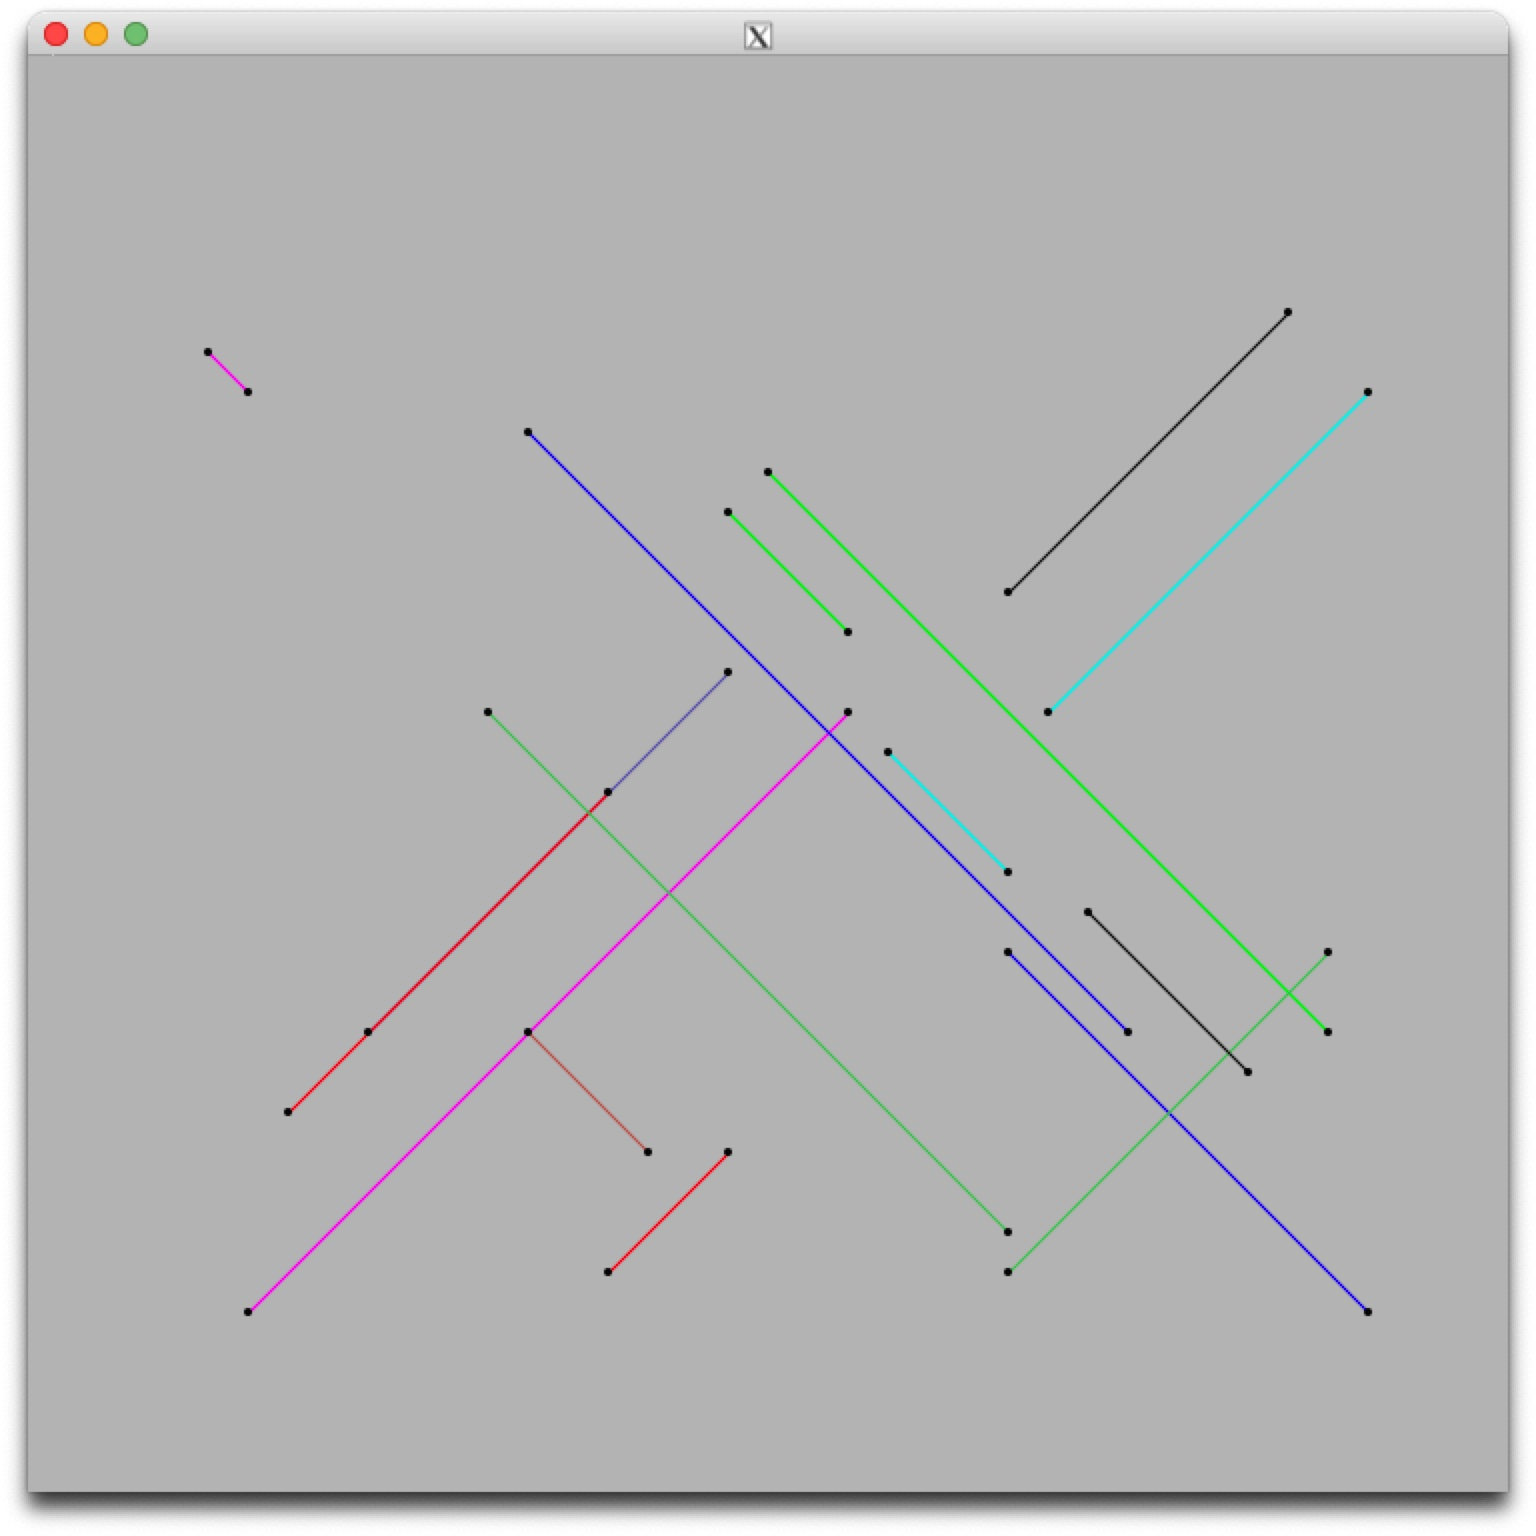
\includegraphics[width=\textwidth]{img/circuit_32x32_16.jpg}
        \label{fig:question1b}
        \subcaption{\scriptsize\texttt{java WireGrapher ./inputs/testinput/circuit\_32x32\_16.txt}}
    \end{minipage}
    \hspace{0.2cm}
    \begin{minipage}{0.3\textwidth}
        \centering
        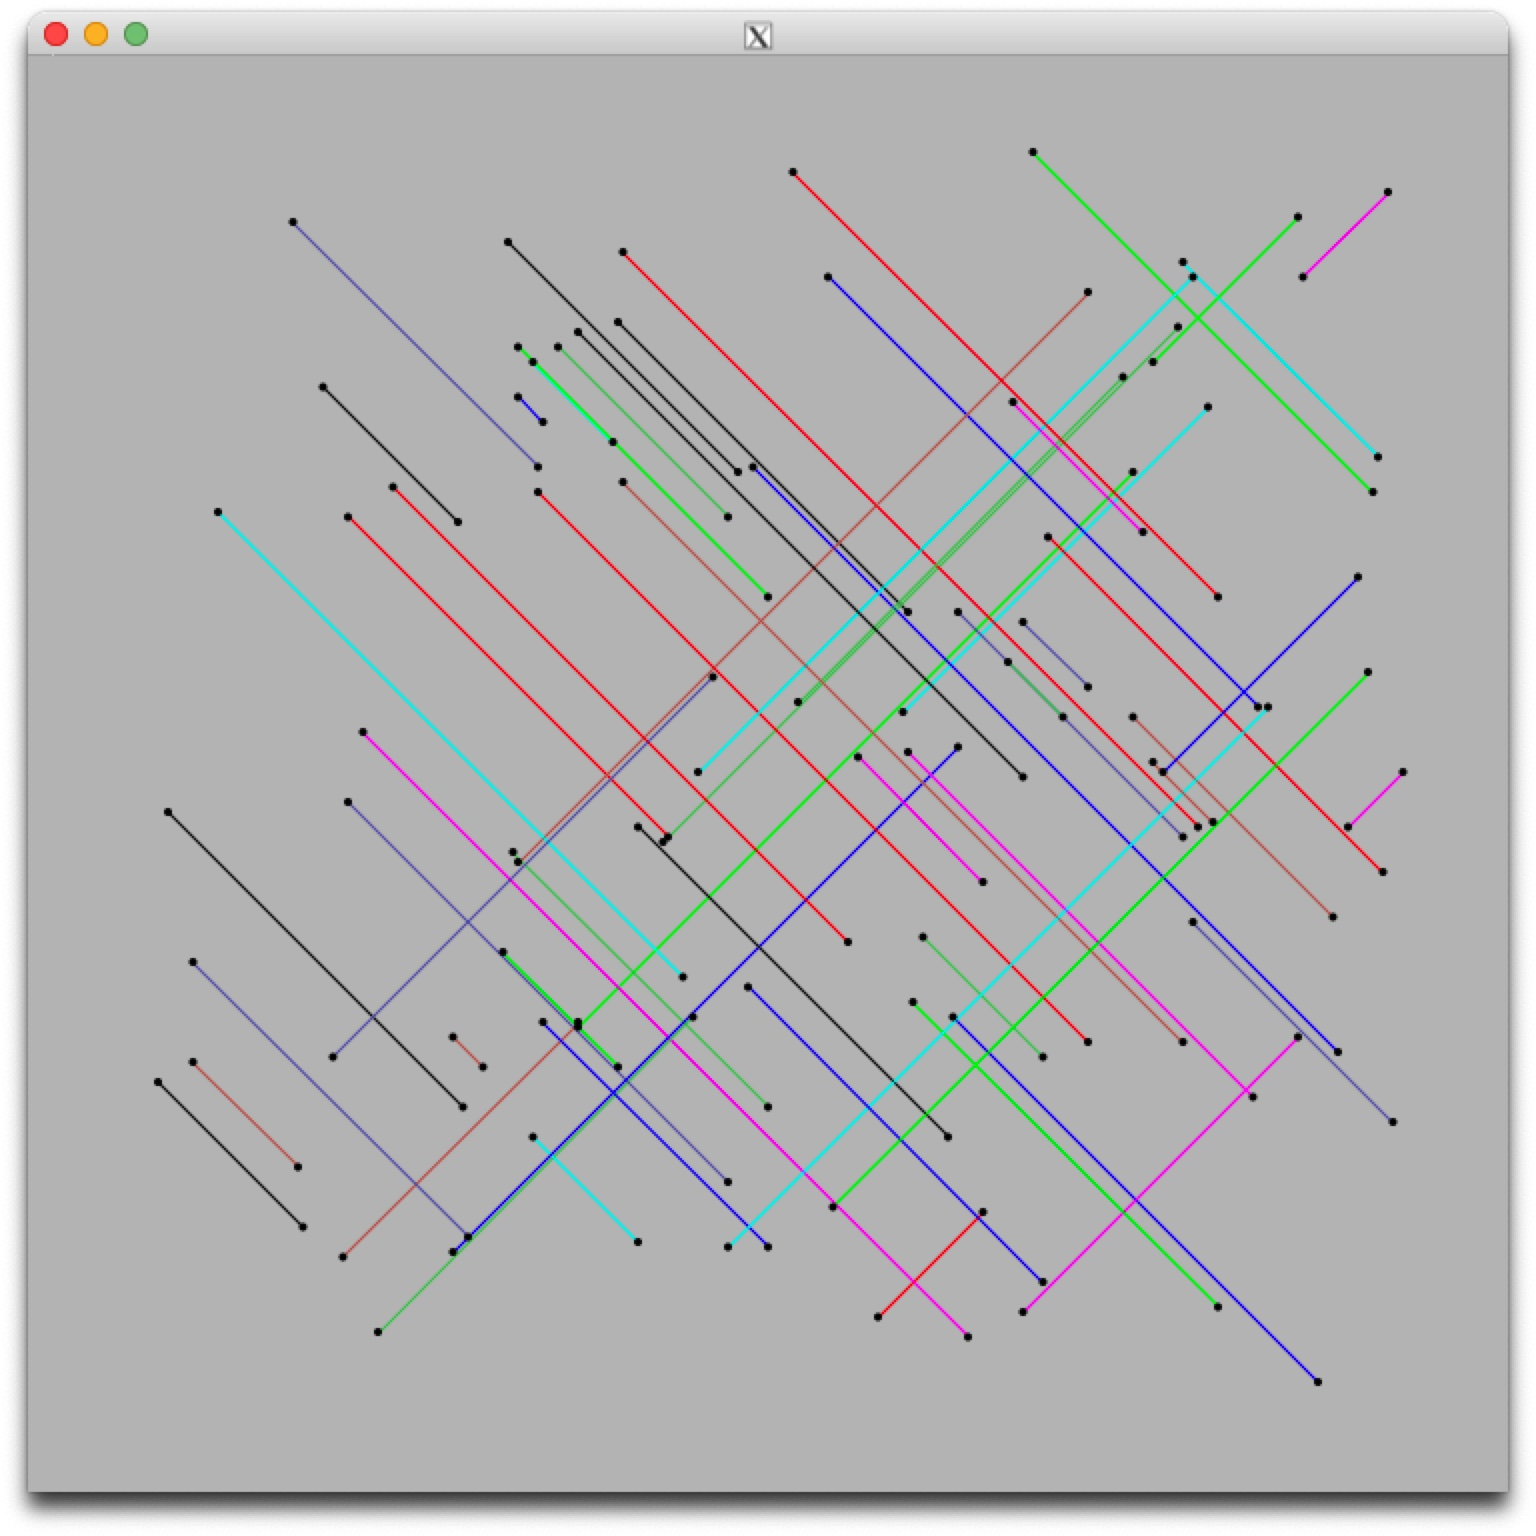
\includegraphics[width=\textwidth]{img/circuit_256x256_64.jpg}
        \label{fig:question1b}
        \subcaption{\scriptsize\texttt{java WireGrapher ./inputs/testinput/circuit\_256x256\_64.txt}}
    \end{minipage}
    \hspace{0.2cm}
    \begin{minipage}{0.3\textwidth}
        \centering
        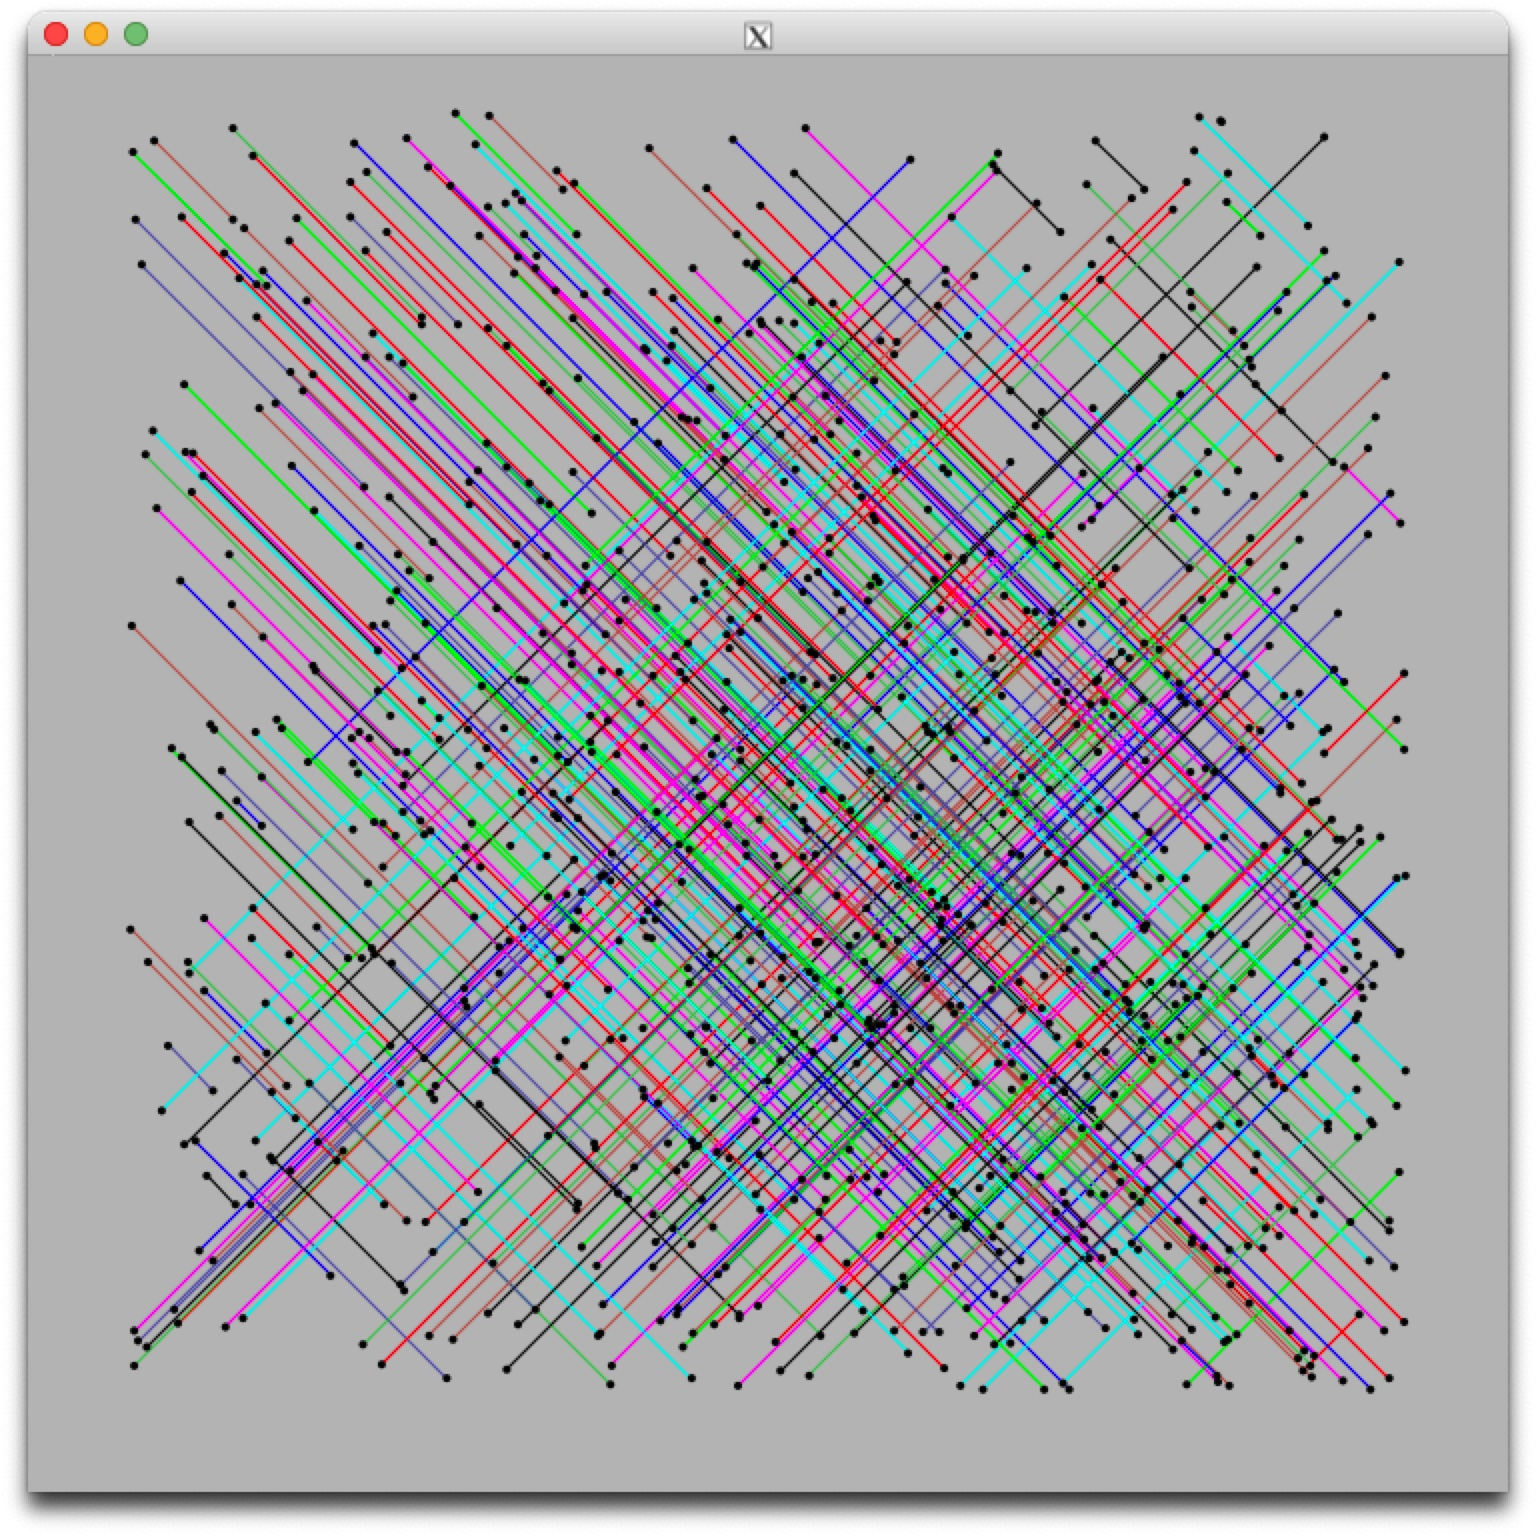
\includegraphics[width=\textwidth]{img/circuit_1024x1024_512.jpg}
        \label{fig:question1b}
        \subcaption{\scriptsize\texttt{java WireGrapher ./inputs/testinput/circuit\_1024x1024\_512.txt}}
    \end{minipage}
\end{figure}

\vspace{0.5cm}
\textbf{Note:} \\
In this assignment, I ignore Simulated Annealing to simplify the problem. I did not benchmark the cache performance as \texttt{perf} not installed on my Andrew machine. \\
Besides, I do not have the access to the PSC machines, so I also skip that section.

\begin{questions}
    \question
    \subsection*{Design and performance debugging for my Within-Wires approach (20 pts)}

    \begin{enumerate}[label=\roman*.]
        \item This problem requires us to minimize the overall total cost (the sum of the squares over all matrix elements),
              while speedup the programs, taking advantage of parallelism across multiple processor cores.

        \item The implementation of VLSI wire routing problem solver.

              \begin{lstlisting}[]
int main(int argc, char *argv[]) {
    // variable declarations...
    parse_arguments(argc, argv, input_filename, num_threads, SA_prob, SA_iters, parallel_mode, batch_size);

    Logger logger;
    WireRouter router(parallel_mode);

    /* Initialize any additional data structures needed in the algorithm */
    initialize_routing(input_filename, dim_x, dim_y, num_wires, wires, occupancy);
    logger.log_time_message("Initialization");

    // Don't use global variables. Use OpenMP to parallelize the algorithm.
    router.run(wires, occupancy, SA_iters, SA_prob, num_threads);
    logger.log_time_message("Computation");

    wr_checker Checker(wires, occupancy);
    Checker.validate();

    logger.print_occupancy_stats(occupancy);
    logger.persist_wires_occupancy(wires, num_wires, occupancy, dim_x, dim_y, num_threads, input_filename);
}
                \end{lstlisting}

              \begin{figure}[h!]
                  \centering
                  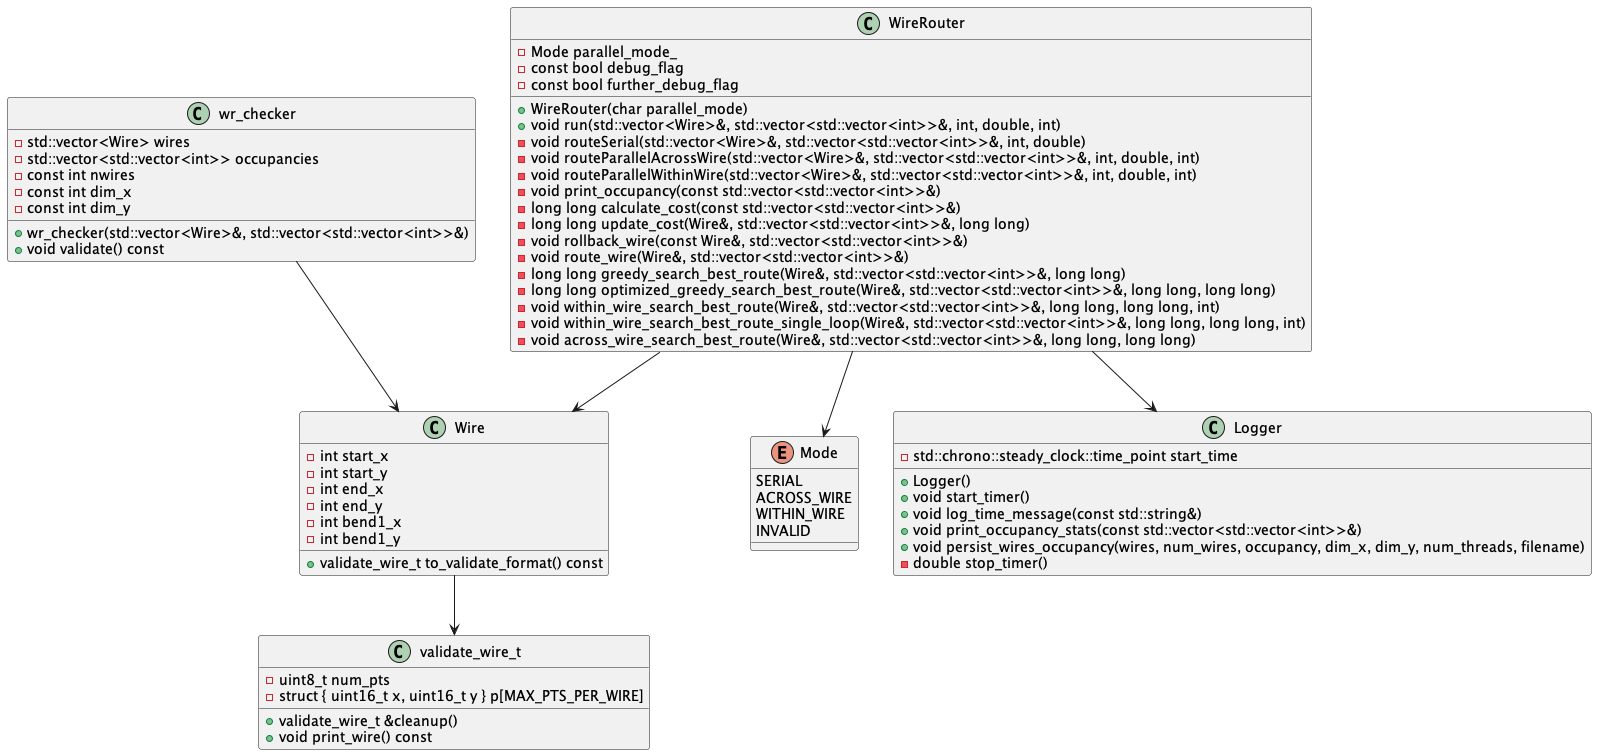
\includegraphics[width=\textwidth]{./img/structure.png}
                  \caption{Structure of the Wire Routing Solver.}
                  \label{fig:structure}
              \end{figure}

        \item I implement the serial version of the algorithm first, and then parallelize it using OpenMP.
              %   The pseudocode is as follows.

              \begin{lstlisting}[]
function routeSerial(wires, occupancy, SA_iters, SA_prob):
    for iteration in range(0, SA_iters):
        for wire in wires:
            // Wire endpoints are on a straight line, skip bend calculations
            if wire.start_x == wire.end_x or wire.start_y == wire.end_y:
                continue
            end if
            rollback_wire(wire, occupancy)  // Remove wire from occupancy grid
            new_wire = copy(wire)
            greedy_search_best_route(new_wire, occupancy, minimum_cost)
            route_wire(new_wire, occupancy)  // Place the new wire on the grid
            wire = new_wire
        end for
    end for
                \end{lstlisting}

              At first, I did rollback and re-routed the wires, and re-calculated the cost from the occupancy matrix while doing the greedy search, which is inefficient.
              I realized that \texttt{rollback\_wire()} and \texttt{route\_wire()} are $O(\Delta x + \Delta y)$, but the calculate cost is $O(\Delta m \times \Delta n)$ (running in greedy searching along horizontal and vertical directions).,
              thus further optimizing the algorithm by alternating the cost calculation with online calculation with reading the occupancy matrix during the search. \\

              \begin{quote}
                  \hspace{-1.5cm} What approaches did you take to parallelize the algorithm?
              \end{quote}

              Then, after the serial version, I parallelize the algorithm with the within wire approach.
              Within wire approach divided the work of routing one wire into multiple threads, where each thread is responsible for routing one path ($\Delta x + \Delta y$ in total) for this wire. \\

              \begin{quote}
                  \hspace{-1.5cm} Include your reasoning for your final implementation choices, including any graphs or tables
                  that helped you make your decisions.
              \end{quote}
              To increase the parallelism and make the threads as busy as possible, I use dynamic scheduling.
              Then, I either merge the greedy searching logic into one loop or use "omp for" to divide the work into several parts to balance the workload. \\
              I tried omp sections as well, but it turns out to be inefficient when I only have two searching directions (horizontal and vertical).\\

              \begin{quote}
                  \hspace{-1.5cm} Where is the synchronization in your solution? Did you do anything to limit the overhead of
                  synchronization?
              \end{quote}

              Use \texttt{\#pragma omp critical} to split the critical sections and synchronize the threads. \\
              Limit the private variables to reduce the overhead. \\

              \begin{quote}
                  \hspace{-1.5cm} Why do you think your code is unable to achieve perfect speedup? (Is it workload imbalance?
                  communication/synchronization? data movement?)
              \end{quote}
              There is necessary communication and synchronization cost.
              For the private variables of each thread, they need to synchronize when they select the best wire. \\

              \begin{quote}
                  \hspace{-1.5cm} At high thread counts, do you observe a drop-off in performance? If so (and you may not), why
                  do you think this might be the case?
              \end{quote}

              No (within 8 threads). The thread number is not the bottleneck and the overhead of more threads can be reduced by the shared memory and paid off by the speedup of the algorithm.
              Besides, I use dynamic scheduling to keep all threads busy and fully utilize the multi-thread parallelism.

    \end{enumerate}



    % \begin{enumerate}[label=\roman*.]
    % \item This type of problem decomposition is referred as Spatial Decomposition since different spatial regions of the image are computed by different processors.

    %       Note that the processor (eight 3.2 GHz Intel Core i7 processors) only has 8 cores, but each core supports two hyper-threads.
    % \item We partition the image generation work into the appropriate number of horizontal blocks.

    %       \begin{itemize}[label=$\circ$]
    %           \item Speedup is not linear in the number of cores used.
    %           \item The workload is not necessarily evenly distributed among the threads.
    %           \item My measurements show that the elapsed time is not same for each thread, which explains the non-linear speedup due to non-evenly workload.
    %       \end{itemize}

    %       \vspace{0.3cm}      

    % \item Modify the mapping of work to threads to improve speedup to almost 8x on the first two
    %       views of the Mandelbrot set.

    %       To decompose the work into row-wise blocks, we can assign each thread to compute a row of the image.
    %       This way, the workload is more evenly distributed among the threads, we could reach speedup around 7.40x \textasciitilde 7.53x.
    %       For view 1, the speedup from 4 to 8 threads is from 3.81x to 7.47x, but from 8 to 16 threads, the speedup is from 7.47x to 7.40x.
    %       For view 2, the speedup from 4 to 8 threads is from 3.72x to 7.29x, but from 8 to 16 threads, the speedup is from 7.29x to 7.28x.

    %       In my decomposition policy, the scaling behavior are different from 4 to 8 threads and 8 to 16 threads, which indicates 4 to 8 threads speedup is almost linear because all threads have access to independent physical cores. However, 8 to 16 threads speedup is not linear because the threads are sharing the same physical core due to hyper-threading.
    % \end{enumerate}

    \question
    \subsection*{Design and performance debugging for my Across-Wires approach (40 pts)}
    For the Across-Wires approach, I divided the work of all wires to different threads at the same time.
    Each thread will be assigned to route a wire, and each thread will do their own greedy search for the best path of this wire. \\

    They have the shared occupancy matrix, and they need to synchronize when they try to update the matrix (\texttt{route\_wire} and \texttt{rollback\_wire}). \\

    % TO be honest, it seems easier than the within wires approach due to my serial implementation.

    \begin{lstlisting}[]
function routeParallelAcrossWire(wires, occupancy, SA_iters, SA_prob, num_threads):
    omp_set_num_threads(num_threads);    
    for iteration in range(0, SA_iters):
        
    #pragma omp parallel for default(shared) schedule(dynamic)
        for wire in wires:
            // Wire endpoints are on a straight line, skip bend calculations
            if wire.start_x == wire.end_x or wire.start_y == wire.end_y:
                continue
            end if

            #pragma omp critical
            rollback_wire(wire, occupancy)  // Remove wire from occupancy grid
            
            new_wire = copy(wire)
            across_wire_search_best_route(new_wire, occupancy, minimum_cost)

            #pragma omp critical
            route_wire(new_wire, occupancy)  // Place the new wire on the grid
            
            wire = new_wire
        end for
    end for
                        \end{lstlisting}

    To be honest, I think the synchronization here is not fully correct and safe, as read and write the matrix from different threads might mess up.
    However, it passed the correctness test, and here is an explanation from piazza Fall 2024 @215. \\

    \begin{quote}
        \hspace{-1.0cm} "I had the same question during my implementation but after actually trying to use synchronization, I noticed that the cost without synchronization is actually lower than with synchronization, and faster too. I think the reason is that yes, reading when others are not finished updating will potentially mess up the actual cost of the path, but this cost is accounting for a partial wire. If the other workers completes that wire, then this routing might be better because it tries to avoid at least part of the other wire. Also, each iteration doesn't find the optimal path but just an approximation. It's likely that even if some partial wires mess up the cost calculation, the result is still going to be a good enough path. Hope this helps."
    \end{quote}
    \newpage

    % \begin{enumerate}[label=\roman*.]
    %     \item The implementation of \texttt{cudaScan()} (to get exclusive prefix sum) has been completed and passed the correctness test.

    %           \begin{lstlisting}[]
    %             \end{lstlisting}
    %     \item The implementation of \texttt{find\_peaks()} (to get exclusive prefix sum) has been completed and passed the correctness test.
    % \item The implementation of \texttt{clampedExpVector()} should work with any combination of input
    %       array size N and vector width W.
    % \item Run \texttt{./vrun -s 10000} and sweep the vector width over the values {2, 4, 8, 16, 32}.
    %       Record the resulting vector utilization.

    %       \begin{table}[ht]
    %           \centering
    %           \scriptsize
    %           \begin{tabular}{|c|c|c|c|c|c|}
    %               \hline
    %               VECTOR\_WIDTH W           & 2            & 4            & 8            & 16           & 32           \\ \hline
    %               Total Vector Instructions & 276613       & 141698       & 71238        & 35628        & 17787        \\ \hline
    %               Vector Utilization        & 89.066132 \% & 88.370866 \% & 88.216787 \% & 88.211344 \% & 88.212072 \% \\ \hline
    %           \end{tabular}
    %           \caption{Vector Utilization for Different Vector Widths}
    %       \end{table}

    %       The vector utilization decreases as W increases a bit, but the difference is not significant. The degree of sensitivity the utilization has on the vector width is not very high. \\
    %       The higher W is, the more vector instructions are executed.

    % \item \texttt{arraySumVector()} has been implemented, and the results passed the correctness test as follows.

    %       \includegraphics*[width=0.65\textwidth]{./prog2\_vecintrin/arraySumVector.jpg}
    % \end{enumerate}

    \question
    \subsection*{Routing output (2 pts)}
    Show (graphically) the routing outputs for both parallel versions of your
    program for the medium 4096.txt input circuit, running on 8 processors on the GHC cluster.
    \vspace{-0.2cm}

    \begin{figure}[h]
        \hspace{1cm}
        \begin{minipage}{0.4\textwidth}
            \centering
            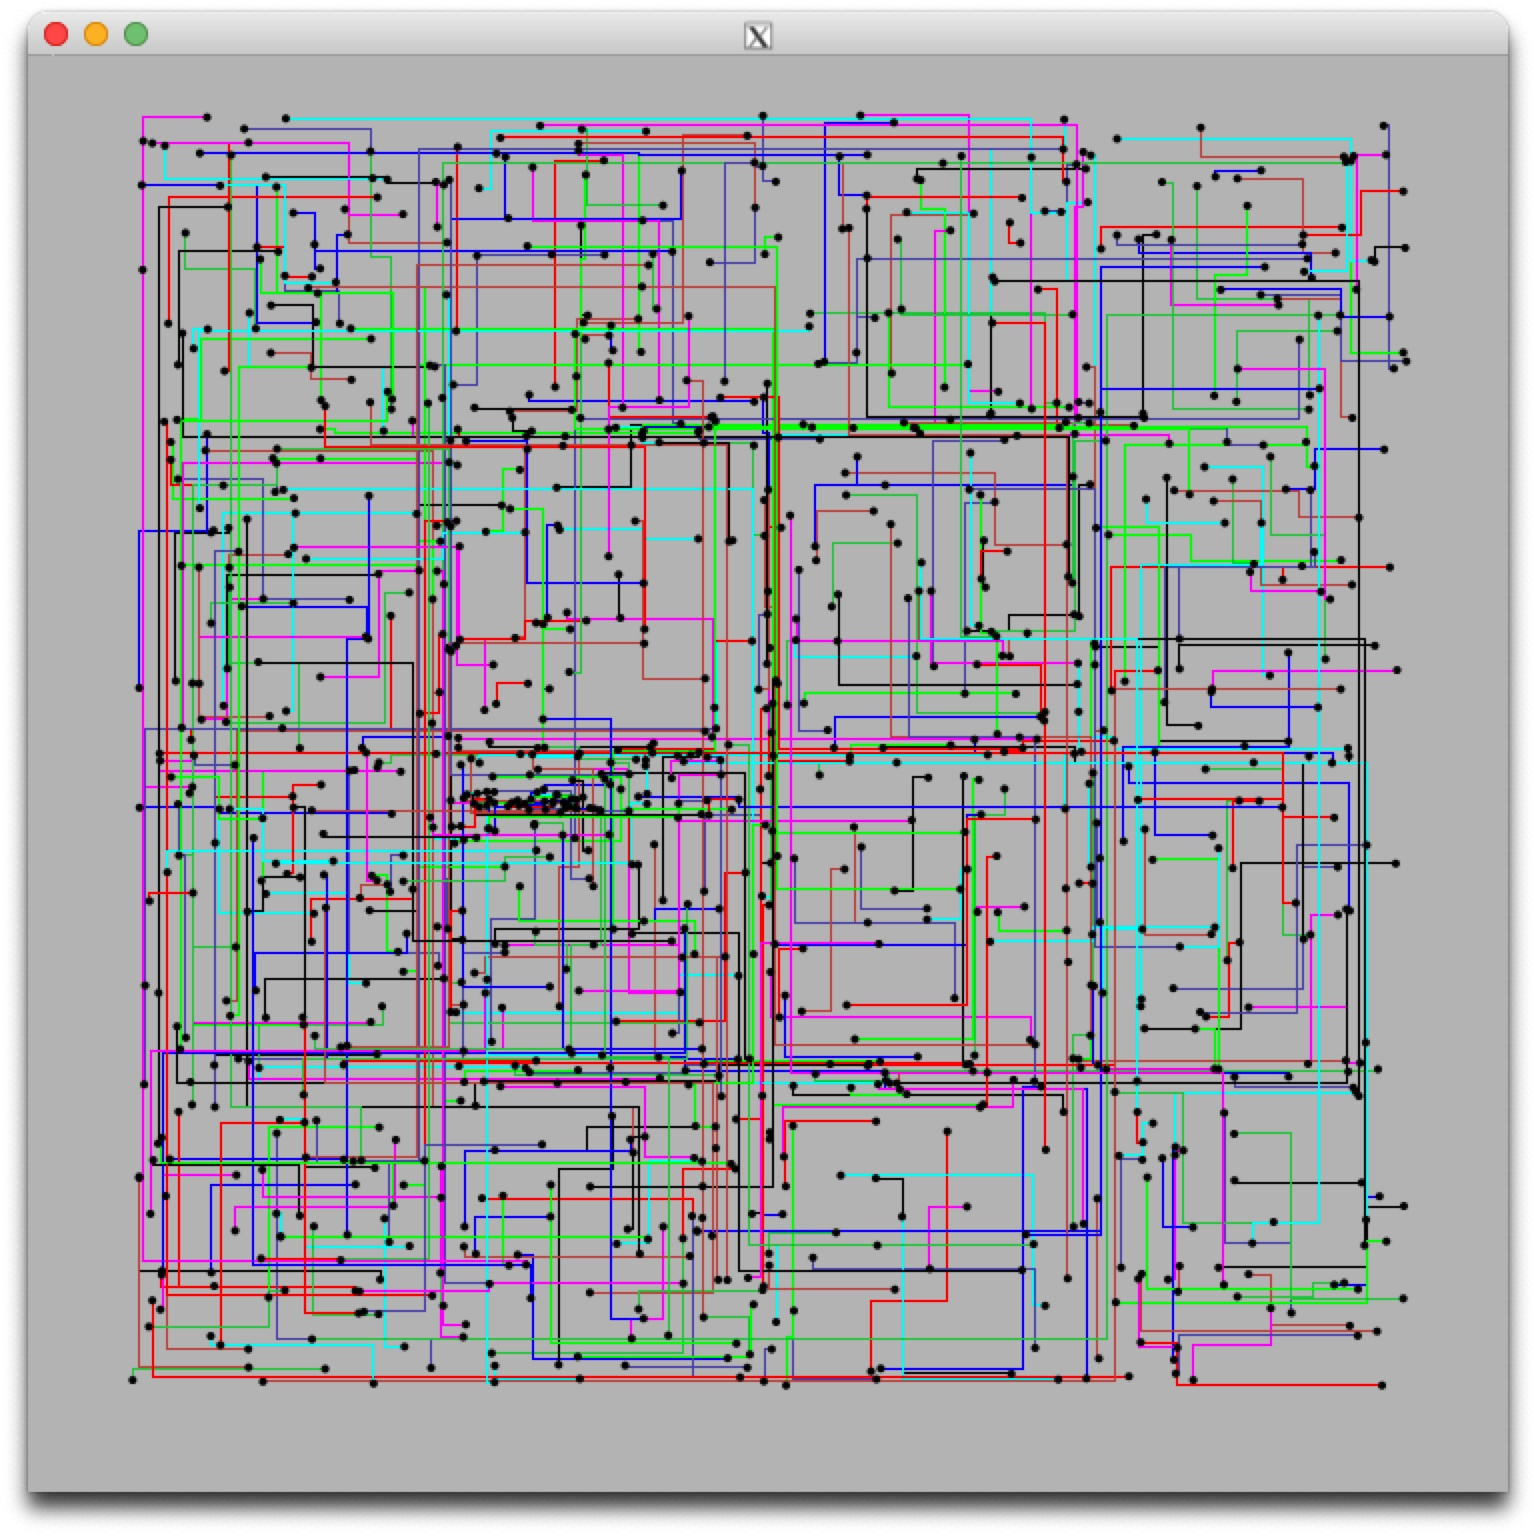
\includegraphics[width=\textwidth]{img/medium_4096_8_A.jpg}
            \label{fig:question1a}
            \vspace{-0.5cm}
            \subcaption{Acorss-Wire \texttt{java WireGrapher ./outputs/timeinput/medium\_4096\_wires\_8.txt}}
        \end{minipage}
        \hspace{0.2cm}
        \begin{minipage}{0.4\textwidth}
            \centering
            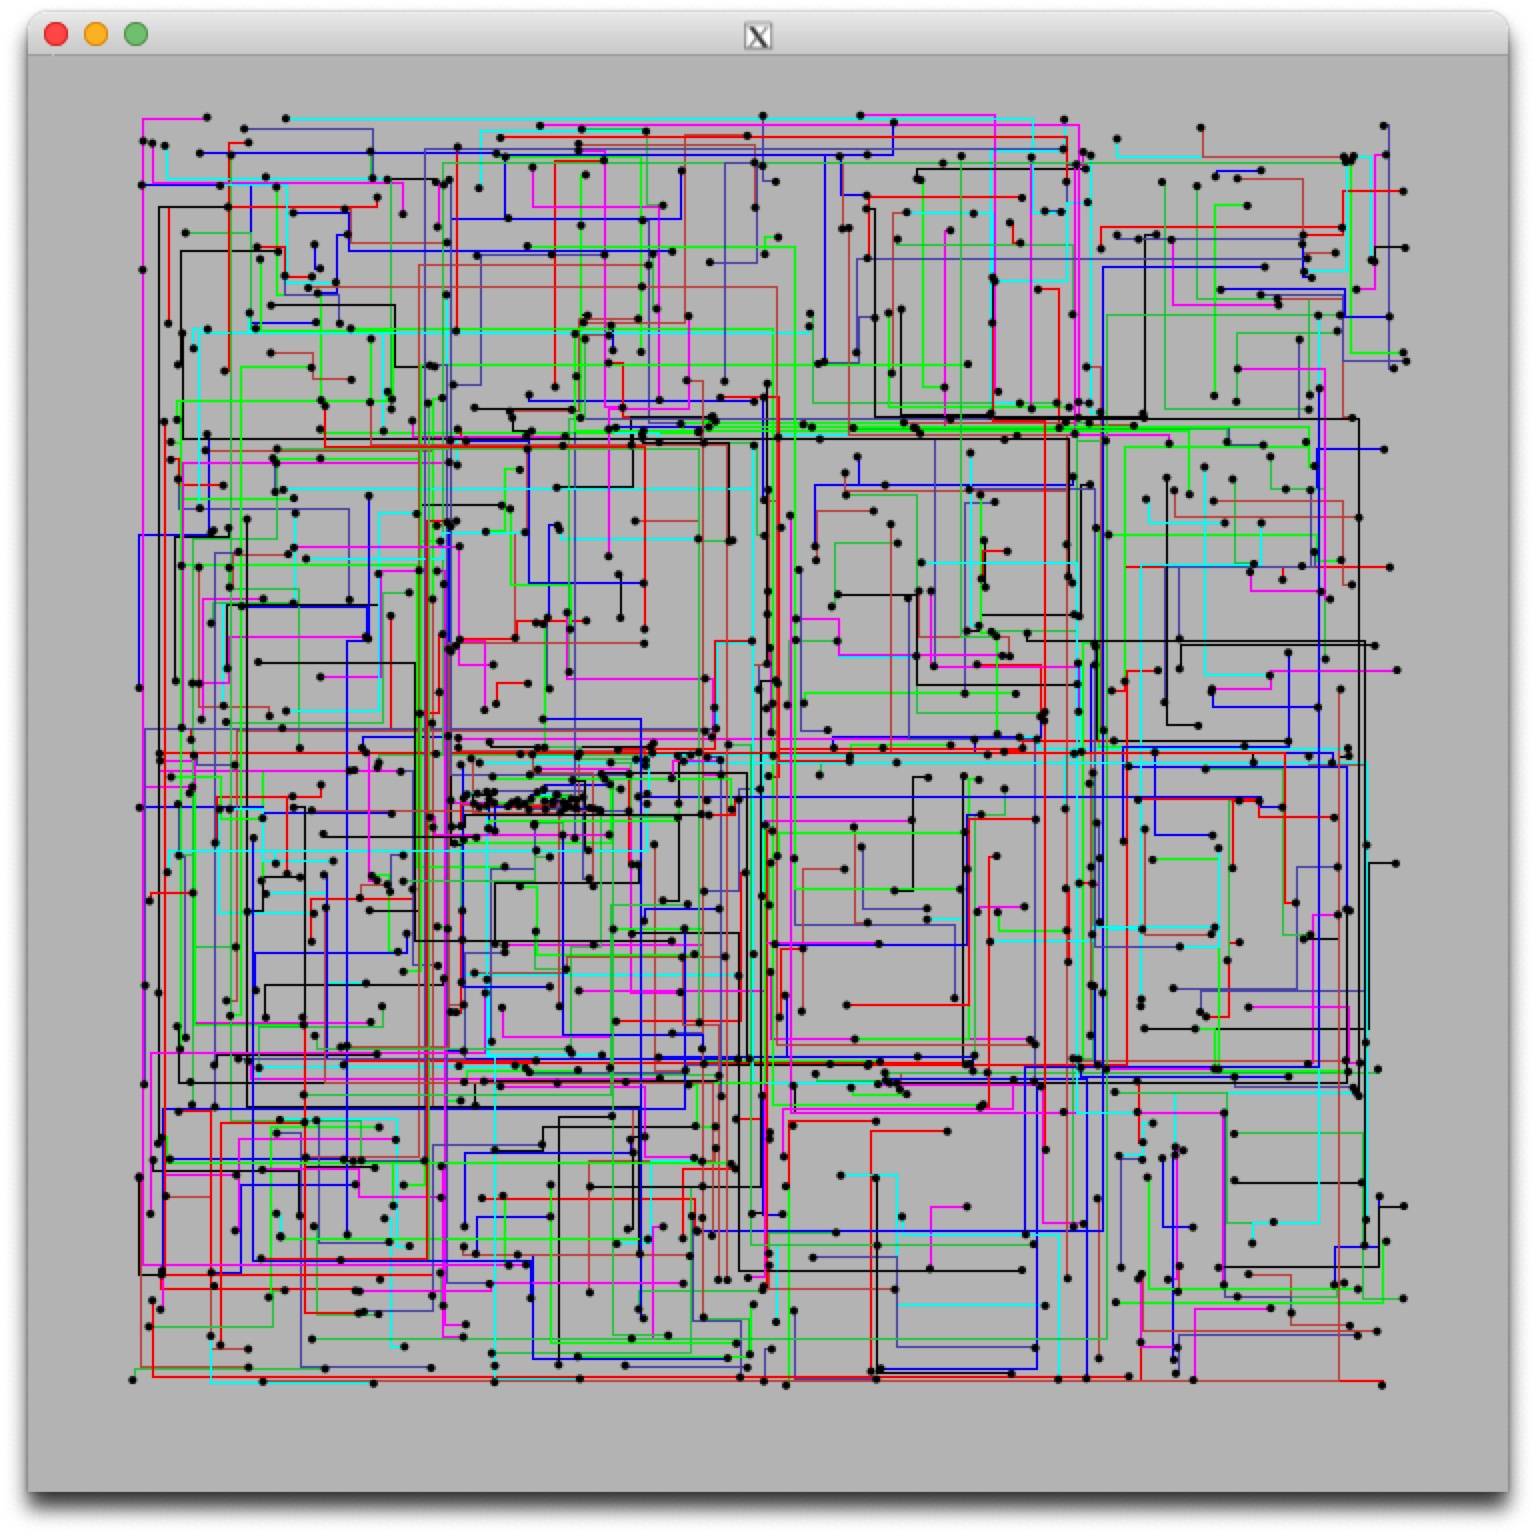
\includegraphics[width=\textwidth]{img/medium_4096_8_W.jpg}
            \label{fig:question1b}
            \vspace{-0.5cm}
            \subcaption{Within-Wire \texttt{java WireGrapher ./outputs/timeinput/medium\_4096\_wires\_8.txt}}
        \end{minipage}
    \end{figure}
    % \begin{enumerate}[label=\roman*.]
    %     \item First, given starter code.
    %           %   \begin{figure}[h]
    %           %       \begin{minipage}{0.45\textwidth}
    %           %           \centering
    %           %           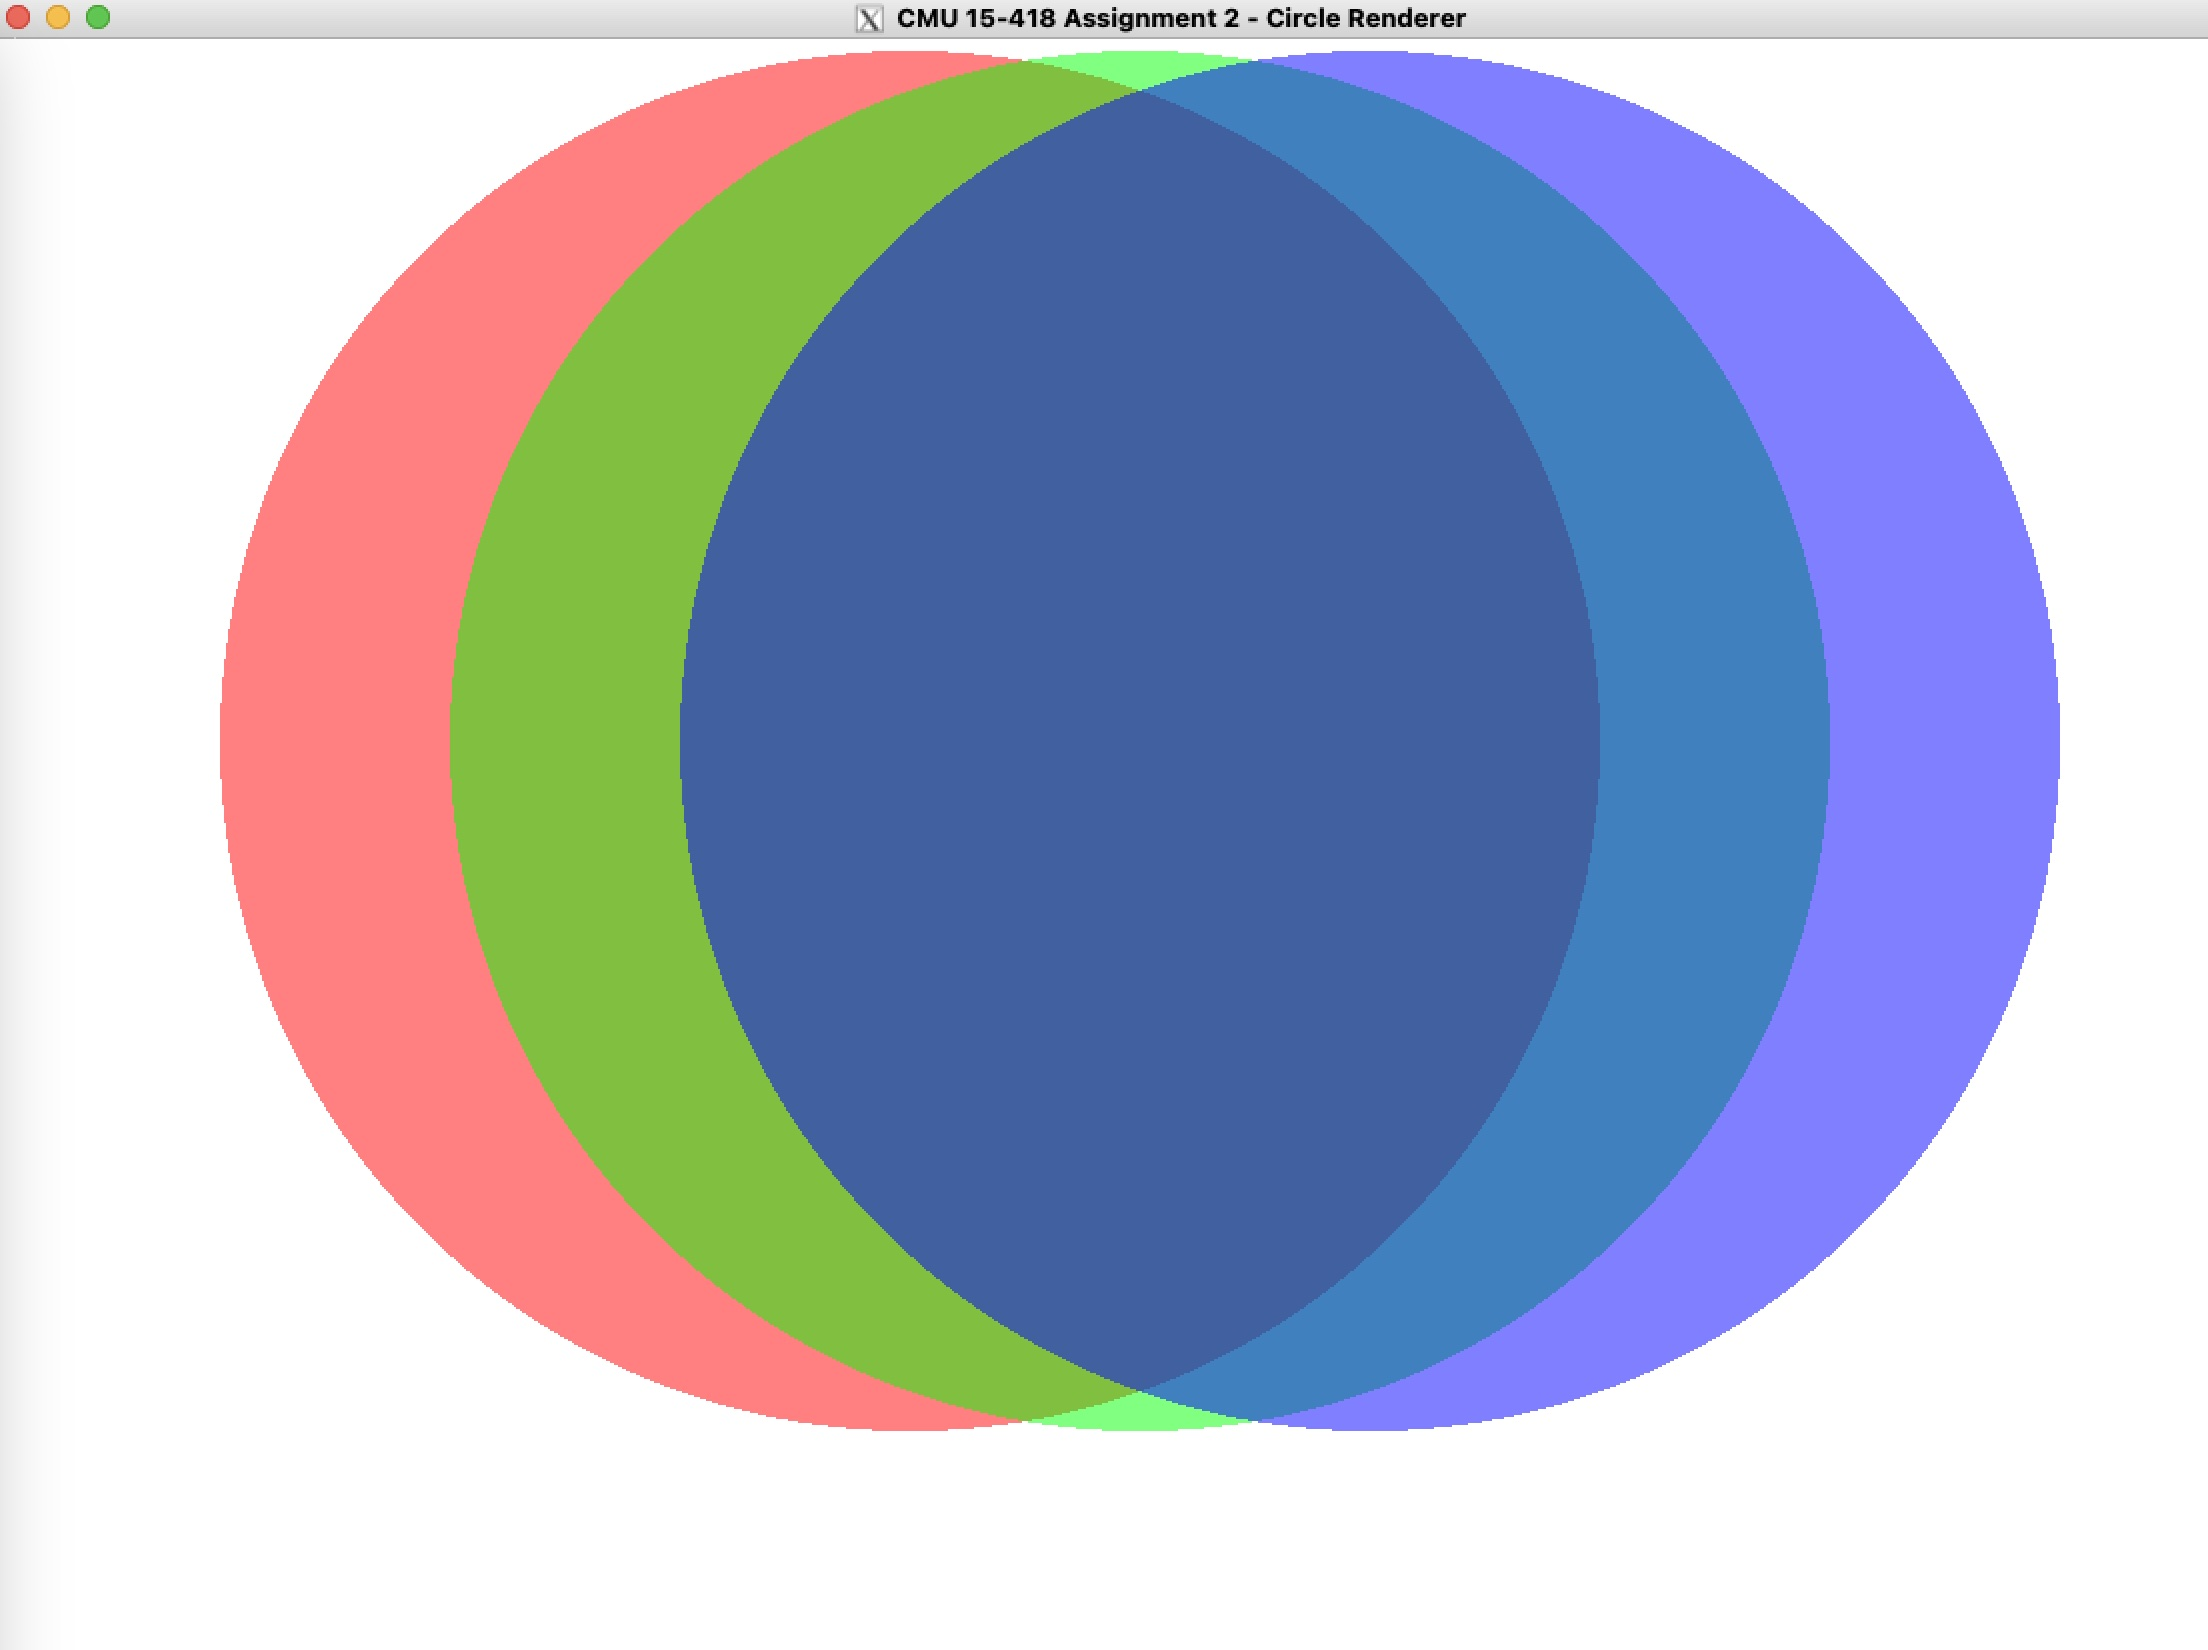
\includegraphics[width=\textwidth]{img/render_rgb.jpg}
    %           %           \label{fig:question3b}
    %           %           \caption{\texttt{./render rgb}}
    %           %       \end{minipage}
    %           %       \hspace{1cm}
    %           %       \begin{minipage}{0.45\textwidth}
    %           %           \centering
    %           %           
\includegraphics[width=\textwidth]{img/render_snow.jpg}
    %           %           \label{fig:question3b}
    %           %           \caption{\texttt{./render snow}}
    %           %       \end{minipage}
    %           %       %   \hspace{-0.5cm}
    %           %       %   \begin{minipage}{0.5\textwidth}
    %           %       %   \end{minipage}
    %           %   \end{figure}
    % \end{enumerate}

    \question
    \subsection*{Experimental results from the GHC machines (20 pts)}
    \begin{enumerate}[label=\roman*.]
        \item For each of these experiments, please
              collect and present data for 1, 2, 4, 8, \sout{and 16} threads for each experiment while running on the
              GHC cluster (ghcX, where X is between 26 and 86). Perform the analysis below for both of your
              parallelization strategies: \textbf{within-wires and across-wires}
        \item Speedup graphs: Show a plot of the \sout{Total Speedup and} Computation Speedup vs. Number of
              Processors (Nprocs). % Discuss these results, including any non-ideal behaviors.
        \item \sout{Cache misses.} (skipped)

              \captionsetup{font=small, labelfont=bf}
              \begin{table}[h!]
                  \centering
                  \caption{Performance Comparison (Time in Seconds \& Computation Speedup Factors) for VLSI Wire Routing}
                  \begin{tabular}{@{}llcccc@{}}
                      \toprule
                      \textbf{Data/TXT File}            & \textbf{Method} & \textbf{Single Thread} & \textbf{2 Threads} & \textbf{4 Threads} & \textbf{8 Threads} \\
                      \midrule
                      \multirow{2}{*}{easy\_4096}       & within          & 0.7519 (1.00x)         & 0.4412 (1.7x)      & 0.2757 (2.73x)     & 0.1769 (4.25x)     \\
                                                        & across          & 0.7465 (1.00x)         & 0.4153 (1.8x)      & 0.2424 (3.08x)     & 0.1610 (4.64x)     \\
                      \midrule
                      \multirow{2}{*}{medium\_4096}     & within          & 11.7119 (1.00x)        & 6.2040 (1.89x)     & 3.4459 (3.4x)      & 1.8175 (6.44x)     \\
                                                        & across          & 11.5672 (1.00x)        & 5.9062 (1.96x)     & 3.0439 (3.8x)      & 1.5926 (7.26x)     \\
                      \midrule
                      \multirow{2}{*}{hard\_4096}       & within          & 14.8109 (1.00x)        & 7.9029 (1.87x)     & 4.4132 (3.36x)     & 2.335 (6.34x)      \\
                                                        & across          & 14.7000 (1.00x)        & 7.4589 (1.97x)     & 3.8410 (3.83x)     & 2.0189 (7.28x)     \\
                      \midrule
                      \multirow{2}{*}{extreme\_4096}    & within          & 66.0754 (1.00x)        & 38.6065 (1.71x)    & 23.7005 (2.79x)    & 13.0250 (5.07x)    \\
                                                        & across          & 65.5949 (1.00x)        & 33.2610 (1.97x)    & 17.1295 (3.83x)    & 8.8578 (7.41x)     \\
                      \midrule
                      \multirow{2}{*}{impossible\_4096} & within          & 509.445 (1.00x)        & 285.091 (1.94x)    & 172.879 (3.45x)    & 99.168 (7.01x)     \\
                                                        & across          & 514.908 (1.00x)        & 264.419 (1.95x)    & 135.083 (3.40x)    & 79.163 (6.76x)     \\
                      \bottomrule
                  \end{tabular}
                  \label{tab:wire_routing_comparison}
              \end{table}
        \item Computation Speedup Comparison Graph.

              \includegraphics*[width=0.9\textwidth]{./img/speedup_comparison.png}
    \end{enumerate}

    \newpage
    \question
    \subsection*{Sensitivity studies on the GHC machines (8 pts)}
    \begin{enumerate}[label=\roman*.]
        \item For these experiments on the GHC machines,
              collect numbers for just your \textbf{across-wires} approach, using just 1 and 8 threads.

        \item \sout{Sensitivity to the probability of choosing a random route} (skipped)
        \item Sensitivity to the problem size: Show a plot of the Computation Speedup on 8 threads with
              respect to 1 thread where the input problem size is varied using the different input files in
              /code/inputs/problemsize directory. In particular, we are focusing on differences in
              grid sizes and numbers of wires. % Please discuss the impact of varying the problem size on performance, explaining any effects that you see.

              \captionsetup{font=small, labelfont=bf}
              \begin{table}[h!]
                  \centering
                  \caption{Sensitivity to the Problem Size based on Across-Wire 8-Threads Computation Speedup <I>}
                  \begin{tabular}{@{}llcccc@{}}
                      \toprule
                      \textbf{Grid Sizes}              & \textbf{hard\_2048} & \textbf{hard\_4096} & \textbf{hard\_8192} \\
                      \midrule
                      \multirow{2}{*}{Speedup Factors} & 2.8548 (1.00x)      & 14.725 (1.00x)      & 114.982 (1.00x)     \\
                                                       & 0.3883 (7.35x)      & 2.0399 (7.22x)      & 15.9210 (7.22x)     \\
                      \bottomrule
                  \end{tabular}
                  \label{tab:wire_routing_comparison}
              \end{table}

              \captionsetup{font=small, labelfont=bf}
              \begin{table}[h!]
                  \centering
                  \caption{Sensitivity to the Problem Size based on Across-Wire 8-Threads Computation Speedup <II>}
                  \begin{tabular}{@{}llcccc@{}}
                      \toprule
                      \textbf{Numbers of Wires}        & \textbf{hard\_4096\_539} & \textbf{hard\_4096\_1123} & \textbf{hard\_4096\_1581} \\
                      \midrule
                      \multirow{2}{*}{Speedup Factors} & 4.9027 (1.00x)           & 14.733 (1.00x)            & 31.790 (1.00x)            \\
                                                       & 0.8387 (5.85x)           & 2.0297 (7.26x)            & 4.3061 (7.38x)            \\
                      \bottomrule
                  \end{tabular}
                  \label{tab:wire_routing_comparison}
              \end{table}
              \includegraphics*[width=0.9\textwidth]{./img/sensitivity_comparison.png}
    \end{enumerate}

    \question
    \subsection*{\sout{Experimental results from the PSC machines (10 pts)}}
    % \begin{enumerate}[label=\roman*.]
    % \end{enumerate}

    % \question
    % \subsection*{Problem 4: Iterative Square Root (10 points)}

    % \begin{enumerate}[label=\roman*.]
    %     \item The sqrt program has been built and run. The speedup due to SIMD (no
    %           tasks) parallelization is 4.77x. The speedup due to multi-core parallelization
    %           is 34.69x.

    %     \item The speedup under different scenarios is as follows.

    %           \begin{table}[ht]
    %               \centering
    %               \scriptsize
    %               \begin{tabular}{|c|c|c|c|}
    %                   \hline
    %                   Case               & Random & initGood & initBad \\ \hline
    %                   SIMD Speedup       & 4.77x  & 6.88x    & 0.95x   \\ \hline
    %                   Multi-Core Speedup & 34.68x & 50.16x   & 6.89x   \\ \hline
    %               \end{tabular}
    %               \caption{Speedup under Different Scenarios}
    %           \end{table}

    %           The \texttt{initGood()} change the value to 2.999. The initialized value of 2.999 could result in the maximum
    %           iteration, and accelerate the paralleled computation to the largest extent. This
    %           modification improves both SIMD and multi-core speedup.

    %           The \texttt{initBad()} change the value to 1.0. The value around 1.0 results in the minimum iteration and the
    %           least absolute computation time. There is not much time to decrease with
    %           parallelism. This modification decreases SIMD and multi-core speedup.

    %           %   \includegraphics*[width=0.65\textwidth]{./prog4\_isqrt/output\_log/speedup_vs_thread_count.png}
    % \end{enumerate}

    % \newpage

    % \question

    % \subsection*{Problem 5: BLAS saxpy (10 points)}

    % The saxpy routine in the BLAS (Basic Linear Algebra Subproblems) library that is
    % widely used (and heavily optimized) on many systems.

    % The \textbf{saxpy} function computes the operation:
    % $\mathbf{r} = a \mathbf{x} + \mathbf{y}$
    % where $a$ is a scalar, and $\mathbf{r}, \mathbf{x}, \mathbf{y}$ are vectors of size $N$ containing single-precision floating-point values.
    % The term \textbf{saxpy} is an acronym for \textbf{"single-precision a x plus y"}.

    % \begin{enumerate}[label=\roman*.]
    %     \item The speedup due to SIMD parallelization is 1x. The speedup from ISPC with tasks is 1.03x.

    %           \captionsetup{font=small, labelfont=bf}
    %           \begin{table}[h!]
    %               \centering
    %               \caption{SAXPY Performance Comparison}
    %               \begin{tabular}{@{}lccc@{}}
    %                   \toprule
    %                   \textbf{Method} & \textbf{Time (ms)} & \textbf{Bandwidth (GB/s)} & \textbf{GFLOPS} \\
    %                   \midrule
    %                   SAXPY Serial    & 11.238             & 26.520                    & 1.780           \\
    %                   SAXPY Streaming & 11.238             & 26.520                    & 1.780           \\
    %                   SAXPY ISPC      & 11.246             & 26.500                    & 1.778           \\
    %                   SAXPY Task ISPC & 10.920             & 27.291                    & 1.831           \\
    %                   \midrule
    %                   \multicolumn{4}{l}{(1.00x speedup from streaming)}                                 \\
    %                   \multicolumn{4}{l}{(1.00x speedup from ISPC)}                                      \\
    %                   \multicolumn{4}{l}{(1.03x speedup from task ISPC)}                                 \\
    %                   \bottomrule
    %               \end{tabular}
    %               \label{tab:saxpy-performance}
    %           \end{table}

    %           I do not think we could achieve linear speedup as the memory bandwidth could be the bottleneck.

    %     \item One value is loaded from vector x \texttt{(N x sizeof(float))}. One value is loaded from vector y \texttt{(N x sizeof(float))}.
    %           One value is written to the result vector  r \texttt{(N x sizeof(float))}.
    %           However, result should be stored in the cache, thus a cache miss will lead to 2 N (read from memory to cache, then back to memory).

    %     \item In addition to the memory bandwidth, the performance of SAXPY might be also limited by poor cache utilization, high cache misses, low pre-fetching efficiency, and the latency of FP operations or DRAM.
    %     \item Improve the performance of saxpy by reducing the memory requirement (modify \texttt{saxpyStreaming()}).
    %           \captionsetup{font=small, labelfont=bf}
    %           \begin{table}[h!]
    %               \centering
    %               \caption{SAXPY Performance Comparison After Streaming}
    %               \begin{tabular}{@{}lccc@{}}
    %                   \toprule
    %                   \textbf{Method} & \textbf{Time (ms)} & \textbf{Bandwidth (GB/s)} & \textbf{GFLOPS} \\
    %                   \midrule
    %                   SAXPY Serial    & 11.280             & 26.421                    & 1.773           \\
    %                   SAXPY Streaming & 8.209              & 36.302                    & 2.436           \\
    %                   SAXPY ISPC      & 11.122             & 26.797                    & 1.798           \\
    %                   SAXPY Task ISPC & 10.900             & 27.342                    & 1.835           \\
    %                   \midrule
    %                   \multicolumn{4}{l}{(1.37x speedup from streaming)}                                 \\
    %                   \multicolumn{4}{l}{(1.01x speedup from ISPC)}                                      \\
    %                   \multicolumn{4}{l}{(1.03x speedup from task ISPC)}                                 \\
    %                   \bottomrule
    %               \end{tabular}
    %               \label{tab:saxpy_comparison}
    %           \end{table}
    % \end{enumerate}

\end{questions}

\end{document}